%% VEIN manuscript --- Springer Nature article class (sn-jnl).
%% Numbered reference style (sn-mathphys-num); referee option = double spacing.
\documentclass[referee,pdflatex,sn-mathphys-num]{sn-jnl}

\usepackage{graphicx}%
\usepackage{multirow}%
\usepackage{amsmath,amssymb,amsfonts}%
\usepackage{amsthm}%
\usepackage{mathrsfs}%
\usepackage[title]{appendix}%
\usepackage{xcolor}%
\usepackage{textcomp}%
\usepackage{manyfoot}%
\usepackage{booktabs}%
\usepackage{algorithm}%
\usepackage{algorithmicx}%
\usepackage{algpseudocode}%
\usepackage{enumitem}%

\theoremstyle{thmstyleone}%
\newtheorem{theorem}{Theorem}%
\newtheorem{proposition}[theorem]{Proposition}%
\theoremstyle{thmstyletwo}%
\newtheorem{example}{Example}%
\newtheorem{remark}{Remark}%
\theoremstyle{thmstylethree}%
\newtheorem{definition}{Definition}%
\newtheorem{assumption}{Assumption}%

\newcommand{\doop}{\mathrm{do}}
\newcommand{\pa}{\mathrm{pa}}
\newcommand{\VaR}{\mathrm{VaR}}
\newcommand{\E}{\mathbb{E}}
\newcommand{\OCCoVaR}{\text{OC-CoVaR}}

\graphicspath{{figures/}}
\raggedbottom

\begin{document}

\title[VEIN: On-Chain Causal Risk Attribution]{VEIN: On-Chain Causal Risk
Attribution for Cryptocurrency Systemic Risk}

\author*[1]{\fnm{Quang-Vinh} \sur{Dang}}\email{vinh.dq4@buv.edu.vn}
\affil*[1]{\orgname{British University Vietnam}, \orgaddress{\city{Hung Yen}, \country{Vietnam}}}

\abstract{Existing causal measures of systemic risk in cryptocurrency markets
infer the contagion graph \emph{statistically} from price returns, using
constraint-based structure learning or directed-information estimation. We
propose VEIN (Verifiable Entity-resolved Interventional/counterfactual Network
risk), a framework that instead treats the \emph{observed} on-chain transaction
graph as the structural backbone of a Pearl-style structural causal model
(SCM): the causal parent set of each economic entity is read off the ledger
rather than estimated from correlations. On this graph VEIN defines an
interventional risk measure (On-Chain Causal CoVaR) through the do-operator and,
to our knowledge, the first counterfactual (Pearl Level-3) systemic-risk
attribution measure in finance, which decomposes a realised loss into the
portion attributable to a specific upstream entity's distress. We implement the
complete pipeline---a four-tier entity-resolution layer over Dune Analytics'
decoded Ethereum tables, the SCM, and the risk measures---and evaluate it on
real on-chain data around the October~2025 cascading liquidation event, the
largest deleveraging episode in crypto history. At the event's native (hourly)
timescale, the observed graph matches or slightly outperforms a price-estimated
Granger graph at predicting the cascade; the OC-CoVaR systemic ranking diverges
from $\Delta$CoVaR and MES (Spearman $\rho=0.52$); the counterfactual measure
attributes concrete loss shares between exchanges; and a battery of
causal-validity checks (placebo/negative controls, unobserved-confounding
robustness values, resolution robustness, and external validity against the
documented event narrative) corroborates the framework. The one assumption that
does \emph{not} survive falsification is that flow \emph{direction} encodes
causal direction: edge reversal barely changes predictions, indicating that
causal information resides in the network's connectivity structure rather than
in flow orientation. We discuss the implications for regulators and the limits
imposed by centralised-exchange opacity. JEL classification: G01, G17, G18, C58.}

\keywords{systemic risk, cryptocurrency, structural causal models,
counterfactual inference, blockchain, CoVaR, contagion}

\maketitle

\section{Introduction}
\label{sec:intro}

On 10--11 October 2025, cryptocurrency markets experienced the largest
deleveraging event in their history: on the order of nineteen billion US
dollars of leveraged positions were liquidated within thirty-six hours. Unlike
the 2022 episodes (Terra/Luna, Celsius, FTX), which were rooted in fundamental
insolvency, the October~2025 cascade was largely \emph{mechanical}: a
mispricing in a centralised exchange's internal valuation engine propagated
into automated liquidations, which in turn forced sales that depressed prices
and triggered further liquidations---a classic funding-liquidity spiral
operating at machine speed. A defining feature was architectural: decentralised
finance (DeFi) lending protocols with transparent, over-collateralised
positions (e.g.\ Aave) emerged with essentially zero bad debt, whereas
centralised-exchange (CEX) risk engines amplified the shock. The synchronised
depeg of the synthetic dollar USDe---which remained fully solvent throughout,
so that the depeg was a pricing and liquidity artefact rather than a
default---is emblematic of this architecture-dependent fragility. Crucially for
risk measurement, the proximate mechanism left a high-resolution footprint
\emph{on chain}: liquidation transfers, collateral movements, and exchange
in/out-flows are all recorded, timestamped to the block, in a public ledger.

Such episodes expose a structural weakness in how systemic risk is measured for
crypto markets. The dominant tools---$\Delta$CoVaR \cite{adrian2016covar},
marginal expected shortfall and SRISK \cite{acharya2017measuring}, and
variance-decomposition connectedness
\cite{diebold2014network,billio2012econometric}---are \emph{associational}:
they quantify co-movement in returns and, as their own authors note, capture an
institution's contribution to system risk ``in a non-causal sense''
\cite{adrian2016covar}. A more recent literature attempts to inject causality.
Causal-NECO VaR \cite{rigana2024neco,rigana2023new} learns a contagion graph
from foreign-exchange returns using the order-independent PC-stable algorithm
\cite{colombo2014order,spirtes2000causation} and computes a value-at-risk from
the resulting SCM. The time-varying directed-information graph (TV-DIG) of
Etesami et al.\ \cite{etesami2023tvdig} builds directed networks---an
information-theoretic generalisation of Granger causality \cite{granger1969}---
across financial sectors including cryptocurrencies. Correlation-network models
such as CoRisk \cite{giudici2018corisk} decompose systemic risk into
idiosyncratic and contagion components. Yet every one of these methods shares a
common limitation: \emph{the causal graph itself is estimated from prices}, so
structure-learning error and data error compound, and no published method
exploits the one data source where the contagion mechanism is \emph{directly
observed}---the blockchain ledger.

Separately, on-chain transaction graphs have been used for prediction and
forensics---``chainlets'' that forecast Bitcoin price and volatility
\cite{akcora2018bitcoin}, address-clustering for anti-money-laundering
\cite{meiklejohn2013fistful,weber2019antimoney}---but always observationally,
explicitly disclaiming a causal-structural interpretation, and never as the
backbone of a systemic-risk measure. And although Pearl's causal hierarchy
\cite{pearl2009causality,pearl2019seven} places counterfactuals (Level~3) above
interventions (Level~2) above association (Level~1), no systemic-risk measure in
finance operates above Level~2. There is, in short, an open intersection:
\emph{an observed-graph SCM for crypto systemic risk, extended to the
counterfactual level}.

\medskip\noindent\textbf{Contribution.} This paper makes three contributions.
\begin{enumerate}[leftmargin=1.4em,itemsep=0.2em]
  \item \textbf{Observed graph as SCM.} We propose VEIN, which treats the
  entity-resolved on-chain transaction graph as the structural backbone of a
  Pearl SCM. The causal parent set $\pa(i)$ of each entity is \emph{read off the
  ledger}, not inferred from price correlations. The temporal precedence of
  on-chain transactions (guaranteed by block timestamps) supplies an
  identification advantage unavailable to price-based methods.
  \item \textbf{Counterfactual systemic risk.} We define On-Chain Causal CoVaR,
  an interventional (Level-2) measure via the do-operator, and a counterfactual
  (Level-3) attribution measure that decomposes a realised loss into the share
  attributable to a specific upstream entity, via the standard
  abduction--action--prediction procedure.
  \item \textbf{End-to-end implementation and honest evaluation.} We implement
  the full pipeline---including a four-tier entity-resolution layer over real
  decoded Ethereum data---and evaluate it on the October~2025 event, comparing
  against price-estimated graphs and standard non-causal baselines, and
  subjecting every causal claim to a falsification and validity battery. We
  report negative results as readily as positive ones.
\end{enumerate}

\medskip\noindent\textbf{Hypotheses.} We organise the evaluation around five
hypotheses (Table~\ref{tab:hyp}), each paired in Section~\ref{sec:results} with
the specific test and falsification criterion that would overturn it.

\begin{table}[t]
\centering
\small
\caption{Hypotheses evaluated in this paper.}
\label{tab:hyp}
\begin{tabular}{@{}p{0.06\linewidth}p{0.84\linewidth}@{}}
\toprule
\textbf{ID} & \textbf{Statement}\\
\midrule
H1 & The observed on-chain flow graph predicts stress propagation more accurately than a graph statistically estimated from price returns.\\
H2 & Reversing flow-edge direction degrades predictive accuracy (flow direction carries causal information; assumption A3).\\
H3 & OC-CoVaR identifies a different set of systemically important entities than $\Delta$CoVaR/MES applied to returns.\\
H4 & The counterfactual measure decomposes the October~2025 losses into mechanically interpretable components.\\
H5 & On-chain composability/collateral edges add loss-attribution information beyond price correlation.\\
\bottomrule
\end{tabular}
\end{table}

The remainder of the paper is organised as follows.
Section~\ref{sec:related} positions VEIN against the causal and on-chain
literatures. Section~\ref{sec:method} develops the framework formally.
Section~\ref{sec:data} describes the data and the entity-resolution pipeline.
Section~\ref{sec:results} reports the empirical evaluation and validity battery.
Section~\ref{sec:discussion} discusses implications, limitations, and
conclusions. An appendix collects implementation details and additional tables.

\section{Related Work and Positioning}
\label{sec:related}

\noindent\textbf{Associational systemic-risk measures.} The canonical
conditional measure is $\Delta$CoVaR \cite{adrian2016covar}, the change in the
value-at-risk of the financial system conditional on an institution being in
distress relative to its median state. The systemic-expected-shortfall family
\cite{acharya2017measuring}---marginal expected shortfall (MES) and the
leverage-adjusted SRISK---measures an institution's losses in the tail of the
system distribution. Connectedness measures based on
forecast-error-variance decompositions \cite{diebold2014network} and on
Granger-causal and correlation networks \cite{billio2012econometric} quantify
spillovers. All are explicitly non-causal: they describe co-movement, not
mechanism.

\medskip\noindent\textbf{Causal value-at-risk.} The closest methodological
precedent is Causal-NECO VaR \cite{rigana2024neco}, which decomposes asset
log-returns into an autoregressive part and an instantaneous contagion part,
learns the causal structure with PC-stable \cite{colombo2014order}, and computes
a Gaussian or Gaussian-copula VaR. It operates at Pearl Levels~1--2 on
foreign-exchange data, assumes no unmeasured confounders, and---decisively for
our purposes---obtains its graph by estimation rather than observation. The
foundational lineage \cite{rigana2023new} combines causal networks with a
structural vector autoregression, drawing on Pearl's framework and the PC
algorithm \cite{spirtes2000causation}. VEIN differs on all three axes: an
observed on-chain graph, crypto entities, and a counterfactual (Level-3)
extension.

\medskip\noindent\textbf{Causal systemic-risk networks including crypto.}
TV-DIG \cite{etesami2023tvdig} is the nearest crypto application: a
nonparametric, time-varying directed-information graph that detects heightened
crypto-to-sector influence around the 2022 stress events. Directed information
generalises Granger causality \cite{granger1969} but is not a Pearl SCM with
do-operator/counterfactual semantics, and it is built from returns, not
on-chain flows.

\medskip\noindent\textbf{On-chain graphs and entity resolution.} Blockchain
transaction graphs have been mined predictively---chainlet subgraphs
forecasting Bitcoin price and volatility \cite{akcora2018bitcoin}---and for
forensics and address clustering, from the multi-input/co-spend heuristics of
\cite{meiklejohn2013fistful} to graph-convolutional anti-money-laundering
classifiers on the Elliptic dataset \cite{weber2019antimoney}. These establish
the resolution machinery VEIN reuses, but none treats the resulting graph as a
causal structure for a systemic-risk measure.

\medskip\noindent\textbf{The gap and our position.} Two specific capabilities
are absent from the published literature as of mid-2026: (i) a counterfactual
(Level-3) VaR/CoVaR measure, and (ii) the use of an observed on-chain
transaction graph as a Pearl SCM for systemic risk. Table~\ref{tab:position}
situates VEIN against the nearest neighbours. We position our contribution
against Causal-NECO VaR (nearest method) and TV-DIG (nearest crypto
application), and re-implement the ``estimated-graph'' approach on our own data
as the head-to-head baseline for H1.

\begin{table}[t]
\centering
\small
\caption{Positioning of VEIN against the nearest prior art.}
\label{tab:position}
\begin{tabular}{@{}p{0.26\linewidth}cccc@{}}
\toprule
\textbf{Method} & \textbf{Graph source} & \textbf{Causal level} & \textbf{Domain} & \textbf{Counterfactual}\\
\midrule
$\Delta$CoVaR \cite{adrian2016covar}     & none (returns)     & assoc.\ (L1) & general & no\\
MES/SRISK \cite{acharya2017measuring}    & none (returns)     & assoc.\ (L1) & general & no\\
CoRisk \cite{giudici2018corisk}          & corr.\ network     & assoc.\ (L1) & credit  & no\\
TV-DIG \cite{etesami2023tvdig}           & estimated (DI)     & Granger     & incl.\ crypto & no\\
Causal-NECO VaR \cite{rigana2024neco}    & estimated (PC)     & SCM (L1--2) & FX      & no\\
\textbf{VEIN (this paper)}               & \textbf{observed} & \textbf{SCM (L1--3)} & \textbf{crypto} & \textbf{yes}\\
\bottomrule
\end{tabular}
\end{table}

\section{The VEIN Framework}
\label{sec:method}

\subsection{Notation and setup}
Let $G=(V,E)$ be a directed, timestamped, dollar-weighted graph whose nodes $V$
are \emph{resolved economic entities} and whose edges $E$ are observed on-chain
flows. For each entity $i$ and discrete time $t$ we define a scalar
\emph{stress state} $S_{i,t}\in\mathbb{R}$ (oriented so that larger means more
distressed), the realised flow $F_{p\to i,t}\ge 0$ from $p$ to $i$ during
period $t$, and an exogenous shock $U_{i,t}$. Table~\ref{tab:notation}
summarises the notation.

\begin{table}[t]
\centering
\small
\caption{Notation.}
\label{tab:notation}
\begin{tabular}{@{}ll@{}}
\toprule
\textbf{Symbol} & \textbf{Meaning}\\
\midrule
$G=(V,E)$ & resolved entity graph (nodes, directed flow edges)\\
$\pa(i)$ & causal parents of $i$ (in-neighbours in $G$)\\
$S_{i,t}$ & stress state of entity $i$ at time $t$ ($z$-scored)\\
$F_{p\to i,t}$ & observed USD flow from $p$ to $i$ in period $t$\\
$U_{i,t}$ & exogenous shock to $i$ at $t$\\
$f_i$ & structural (stress-propagation) function of $i$\\
$L_j$ & loss functional of $j$ over the event window\\
$s^\ast$ & severe-distress intervention level ($95$th pctile)\\
$\Delta_i^{CF}(j)$ & counterfactual loss of $j$ attributable to $i$\\
$RV$ & confounding robustness value\\
\bottomrule
\end{tabular}
\end{table}

\subsection{Structural causal model}
The defining structural equation of VEIN is
\begin{equation}
\label{eq:scm}
S_{i,t} \;=\; f_i\!\Big(S_{\pa(i),\,t-1},\; F_{\pa(i)\to i,\,t},\; U_{i,t}\Big),
\end{equation}
where the parent set
\begin{equation}
\label{eq:parents}
\pa(i) \;=\; \{\,p\in V : (p\to i)\in E\,\}
\end{equation}
is \emph{read directly from the resolved ledger}. This is the central
structural move of the paper: in contrast to
\cite{rigana2024neco,etesami2023tvdig}, $\pa(i)$ is not estimated from data but
observed. The only component requiring statistical estimation is the
stress-propagation function $f_i$. We adopt a ridge-regularised linear
specification,
\begin{equation}
\label{eq:fi}
S_{i,t} \;=\; b_i + \sum_{p\in\pa(i)} a_{ip}\,S_{p,t-1}
            + \sum_{p\in\pa(i)} c_{ip}\,\log\!\big(1+F_{p\to i,t}\big)
            + U_{i,t},
\end{equation}
with parameter vector $\theta_i=(b_i,\{a_{ip}\},\{c_{ip}\})$ estimated by ridge
regression,
\begin{equation}
\label{eq:ridge}
\hat\theta_i \;=\; \arg\min_{\theta_i}\;
\sum_{t} \big(S_{i,t}-f_i(\cdot;\theta_i)\big)^2 + \lambda\big(\|a_{i\cdot}\|_2^2+\|c_{i\cdot}\|_2^2\big),
\end{equation}
on a pre-crisis estimation window, with penalty $\lambda$. The fitted residuals
$\widehat U_{i,t}=S_{i,t}-f_i(\cdot;\hat\theta_i)$ furnish an empirical
distribution of exogenous shocks used below.

\begin{proposition}[Well-posedness of the lagged system]
\label{prop:wellposed}
Because every parent enters \eqref{eq:fi} at lag $t\!-\!1$ in the stress term
and the contemporaneous term depends only on exogenous observed flows
$F_{p\to i,t}$, the map from $(S_{\cdot,t-1},F_{\cdot,t},U_{\cdot,t})$ to
$S_{\cdot,t}$ is explicit. Hence, given an initial state $S_{\cdot,0}$ and a
shock path $\{U_{\cdot,t}\}$, the trajectory $\{S_{\cdot,t}\}_{t\ge 1}$ is
uniquely determined by forward iteration, even when $G$ contains directed
cycles.
\end{proposition}
\begin{proof}[Proof sketch]
At step $t$ the right-hand side of \eqref{eq:fi} for every $i$ references only
quantities indexed at $t\!-\!1$ (parent stress) or exogenous quantities at $t$
(flows, shocks). There is therefore no simultaneity among the time-$t$ stress
variables, and $S_{\cdot,t}$ is computed in one vectorised step from
information available at $t\!-\!1$. Induction on $t$ gives existence and
uniqueness.
\end{proof}

Proposition~\ref{prop:wellposed} is what allows cycles such as
Binance$\leftrightarrow$retail in the observed graph without an equilibrium
fixed-point computation: time, supplied by the ledger, breaks the simultaneity.

\subsection{Identifying assumptions}
\begin{assumption}[Temporal precedence, A1]
A flow $F_{i\to j,t}$ strictly precedes any effect on $j$ at $t'>t$.
\end{assumption}
A1 is supplied \emph{for free} by blockchain immutability and timestamping; it
need not be assumed or tested, unlike Granger-style precedence on price series.

\begin{assumption}[No unobserved common cause for flow edges, A2]
Conditional on the transaction graph up to $t$, an edge $i\to j$ reflects $i$'s
direct economic action on $j$.
\end{assumption}
A2 is defensible because a public ledger captures every fund movement in the
flow mechanism itself. Its principal threat is off-chain activity---most acutely
CEX-internal pricing engines---which we bound through a sensitivity analysis
(Section~\ref{subsec:sens}).

\begin{assumption}[Monotone propagation along flow direction, A3]
Distress at $i$ affects $j$ only through realised flow paths from $i$ to $j$.
\end{assumption}
A3 is the substantive, falsifiable claim of the framework and is tested
directly (H2) by the edge-reversal experiment of Section~\ref{subsec:falsif}.
A1--A2 are structural properties of the data source---the principal
identification advantage over price-based causal discovery, where both the
graph and the equations must be estimated, compounding error.

\subsection{Interventional measure: On-Chain Causal CoVaR}
We summarise an entity's distress over an event window $\mathcal{T}$ by the
non-negative, additive loss functional
\begin{equation}
\label{eq:loss}
L_j \;=\; \sum_{t\in\mathcal{T}} \max\!\big(S_{j,t},\,0\big).
\end{equation}
Applying Pearl's do-operator to~\eqref{eq:scm}, we force entity $i$ into a
distressed state $s^\ast$, severing its own parents, and propagate forward
through the remaining structural equations. The interventional risk measure is
the conditional value-at-risk of $j$'s loss,
\begin{equation}
\label{eq:occovar}
\OCCoVaR_q\big(j \,\big|\, \doop(S_i=s^\ast)\big)
   \;=\; \VaR_q\!\Big(L_j \,\Big|\, \doop(S_i=s^\ast)\Big),
\end{equation}
whose distribution is obtained by Monte-Carlo propagation. For $m=1,\dots,M$ we
draw a shock path $U^{(m)}$ by block-bootstrapping the fitted residuals
$\{\widehat U_{i,t}\}$, simulate \eqref{eq:fi} forward under the intervention to
obtain $S^{(m)}_{j,t}$, and form $L_j^{(m)}$ via \eqref{eq:loss}; the estimator
is the empirical quantile
\begin{equation}
\label{eq:mc}
\widehat{\OCCoVaR}_q\big(j\,|\,\doop(S_i=s^\ast)\big)
   \;=\; \widehat Q_q\big(\{L_j^{(m)}\}_{m=1}^M\big).
\end{equation}
By analogy with $\Delta$CoVaR, the marginal systemic contribution of $i$ to $j$
is
\begin{equation}
\label{eq:deltaoccovar}
\Delta\OCCoVaR_q(j\,|\,i) \;=\;
\OCCoVaR_q\big(j\,|\,\doop(S_i=s^\ast)\big) -
\OCCoVaR_q\big(j\,|\,\doop(S_i=0)\big),
\end{equation}
with $s^\ast$ the $95$th percentile of $i$'s historical stress and the baseline
the median ($0$ after standardisation). We rank entities by their total
\emph{exported} tail risk,
\begin{equation}
\label{eq:exported}
\mathcal{E}(i) \;=\; \sum_{j\ne i}\max\!\big(\Delta\OCCoVaR_q(j\,|\,i),\,0\big).
\end{equation}

\emph{Relation to $\Delta$CoVaR.} Equation~\eqref{eq:deltaoccovar} is the
network-causal analogue of $\Delta$CoVaR \cite{adrian2016covar}: both contrast a
distressed against a median conditioning state. The differences are structural.
$\Delta$CoVaR conditions on a \emph{statistical} event (institution $i$ at its
VaR) and reads off a conditional quantile of returns; $\Delta$OC-CoVaR
conditions on an \emph{intervention} ($\doop(S_i=s^\ast)$) that severs $i$'s own
parents and propagates the shock forward through the observed structural
equations. In the degenerate case of a single edge $i\to j$ with a linear $f_j$
and no further descendants, $\Delta$OC-CoVaR reduces to a quantile shift of $j$
proportional to the structural coefficient $a_{ji}$, mirroring the $\beta_i$
slope in $\Delta$CoVaR; the network generalisation is the sum over all directed
paths from $i$ to $j$.

\subsection{Counterfactual measure: loss attribution}
The counterfactual attribution of $j$'s realised loss to $i$'s distress follows
the three-step procedure \cite{pearl2009causality,pearl2019seven}:
\emph{(i) Abduction}---infer the realised exogenous shocks
$\widehat U_{i,t}=S_{i,t}-f_i(\cdot;\hat\theta_i)$ from observed data;
\emph{(ii) Action}---replace $i$'s realised trajectory by its pre-crisis level,
$\doop(S_i=S_i^{\text{pre}})$, holding all $\widehat U_{k,t}$ ($k\ne i$) fixed;
\emph{(iii) Prediction}---recompute downstream states to obtain
$L_j^{\,\doop(S_i=S_i^{\text{pre}})}$. The attribution and its share are
\begin{equation}
\label{eq:cf}
\Delta_i^{CF}(j) \;=\; L_j^{\text{obs}} - L_j^{\,\doop(S_i=S_i^{\text{pre}})},
\qquad
\text{share}_i(j) \;=\; \frac{\Delta_i^{CF}(j)}{L_j^{\text{obs}}}.
\end{equation}
$\Delta_i^{CF}(j)$ answers: \emph{how much of $j$'s realised loss would not have
occurred had $i$ never become distressed, holding everything else exactly as it
unfolded?} To our knowledge this is the first counterfactual (Level-3)
systemic-risk attribution in finance.

\subsection{Falsification test for A3}
\label{subsec:falsif}
To test, rather than assume, that flow direction carries causal information we
construct three variants of $G$: the true-direction graph, a reversed graph
$G^{\mathrm{rev}}$ (every edge flipped), and a symmetric/undirected graph
$G^{\mathrm{sym}}$. We fit~\eqref{eq:fi} on each over the estimation window and
compare one-step-ahead prediction of event-window stress, scoring the
stress-weighted root-mean-square error
\begin{equation}
\label{eq:rmse}
\mathrm{RMSE} \;=\;
\sqrt{\frac{\sum_{i,t} w_{i,t}\,(\hat S_{i,t}-S_{i,t})^2}{\sum_{i,t} w_{i,t}}},
\qquad w_{i,t}=|S_{i,t}|+0.1 .
\end{equation}
If the true-direction model attains the lowest RMSE this is empirical evidence
for A3; if it does not, A3 must be qualified to specific edge types.

\subsection{Sensitivity to unobserved confounding}
\label{subsec:sens}
Because A2 is not directly testable, we quantify how strong a hidden confounder
(e.g.\ a CEX-internal pricing engine) would have to be to overturn each edge,
using the robustness value of Cinelli and Hazlett \cite{cinelli2020sensitivity}.
For a structural coefficient with $t$-statistic $t$ and $d$ degrees of freedom,
let $f=|t|/\sqrt{d}$; the robustness value for nullifying the estimate is
\begin{equation}
\label{eq:rv}
RV \;=\; \tfrac{1}{2}\Big(\sqrt{f^4+4f^2}-f^2\Big)\in[0,1],
\end{equation}
the share of residual variance an unobserved confounder must explain in
\emph{both} the parent (treatment) and the child (outcome) to drive the
coefficient to zero. Larger $RV$ means a finding is harder to explain away.

\subsection{Baselines}
We compare against three references.
\emph{(i) $\Delta$CoVaR} \cite{adrian2016covar}: estimating the quantile
regression $r^{\mathrm{sys}}_t = \alpha_i + \beta_i\, r_{i,t} + \varepsilon_t$
at level $q$, the measure is
$\Delta\text{CoVaR}_i = \beta_i\big(\VaR_q(r_i)-\VaR_{0.5}(r_i)\big)$.
\emph{(ii) MES} \cite{acharya2017measuring}: the mean return of asset $i$ on the
worst-$q$ system days,
$\text{MES}_i=\E[r_i \mid r^{\mathrm{sys}}\le \VaR_q(r^{\mathrm{sys}})]$.
\emph{(iii) The estimated-graph school}: a Granger graph \cite{granger1969}
(edge $i\to j$ when the lagged return of $i$ significantly predicts that of $j$
in $r_{j,t}=\phi_0+\phi_1 r_{j,t-1}+\phi_2 r_{i,t-1}+u_t$ at level $\alpha$) and
a partial-correlation graph \cite{giudici2018corisk}, both over the same entity
node set and fed through the \emph{same} VEIN machinery so that only the graph
source differs---a like-for-like test of H1.

\subsection{Algorithm}
Algorithm~\ref{alg:vein} summarises the end-to-end procedure.

\begin{algorithm}[t]
\caption{VEIN end-to-end pipeline}
\label{alg:vein}
\begin{algorithmic}[1]
\State \textbf{Input:} decoded on-chain transfers, price/return data, entity labels, event window $\mathcal{T}$
\State $G \gets \textsc{ResolveEntities}(\text{transfers}, \text{labels})$ \Comment{Tiers 0--3, Sec.~\ref{sec:data}}
\For{each entity $i\in V$}
  \State $\hat\theta_i \gets \textsc{FitRidge}\big(\pa(i,G),\, F_{\pa(i)\to i},\, S^{\text{hist}}_i\big)$ \Comment{Eq.~\eqref{eq:ridge}}
\EndFor
\For{each $(i,j)$ of interest}
  \State $\Delta\OCCoVaR_q(j\,|\,i) \gets \textsc{MonteCarloPropagate}(G,\{f_k\},\doop(S_i=s^\ast),M)$ \Comment{Eq.~\eqref{eq:mc}}
\EndFor
\For{each $(i,j)$ in the crisis window}
  \State $\widehat U \gets \textsc{Abduct}(G,\{f_k\},\text{data})$; \enspace
         $L_j^{cf} \gets \textsc{Predict}(G,\{f_k\},\widehat U,\doop(S_i=S_i^{\text{pre}}))$
  \State $\Delta_i^{CF}(j) \gets L_j^{\text{obs}} - L_j^{cf}$ \Comment{Eq.~\eqref{eq:cf}}
\EndFor
\State $G^{\mathrm{rev}},G^{\mathrm{sym}} \gets \textsc{Reverse}(G),\textsc{Symmetrise}(G)$
\State \textsc{CompareAccuracy}$(G,G^{\mathrm{rev}},G^{\mathrm{sym}})$ \Comment{Eq.~\eqref{eq:rmse}}
\State \textbf{Output:} OC-CoVaR ranking, counterfactual attributions, falsification + validity battery
\end{algorithmic}
\end{algorithm}

\section{Data and Entity Resolution}
\label{sec:data}

\subsection{Data sources}
All data are real and obtained from public or keyed APIs;
Table~\ref{tab:data} lists the sources. On-chain flows are queried with SQL
over Dune Analytics' decoded \texttt{erc20\_ethereum.evt\_Transfer} table and
its maintained \texttt{labels.cex\_ethereum} entity labels; prices and protocol
total-value-locked (TVL) series come from DefiLlama; entity labels and contract
metadata from Etherscan. No synthetic data are used. The cascade is directly
visible in the raw data: Figure~\ref{fig:usde} shows the on-chain transfer
volume of the synthetic dollar USDe rising from \$0.75bn on 9~October to
\$3.09bn on 10~October and \$8.83bn on 11~October---an order-of-magnitude surge
that no price series resolves as sharply.

\begin{table}[t]
\centering
\small
\caption{Data sources. All series are real; on-chain flows carry block-level timestamps.}
\label{tab:data}
\begin{tabular}{@{}p{0.27\linewidth}p{0.40\linewidth}p{0.24\linewidth}@{}}
\toprule
\textbf{Layer} & \textbf{Source} & \textbf{Granularity}\\
\midrule
Decoded transfers (ETH) & Dune \texttt{erc20\_ethereum.evt\_Transfer} & per-transfer (block)\\
CEX entity labels & Dune \texttt{labels.cex\_ethereum} & per-address\\
Prices / returns & DefiLlama coins API & hourly \& daily\\
Protocol TVL & DefiLlama & daily\\
Contract metadata & Etherscan v2 & per-contract\\
\bottomrule
\end{tabular}
\end{table}

\begin{figure}[t]
\centering
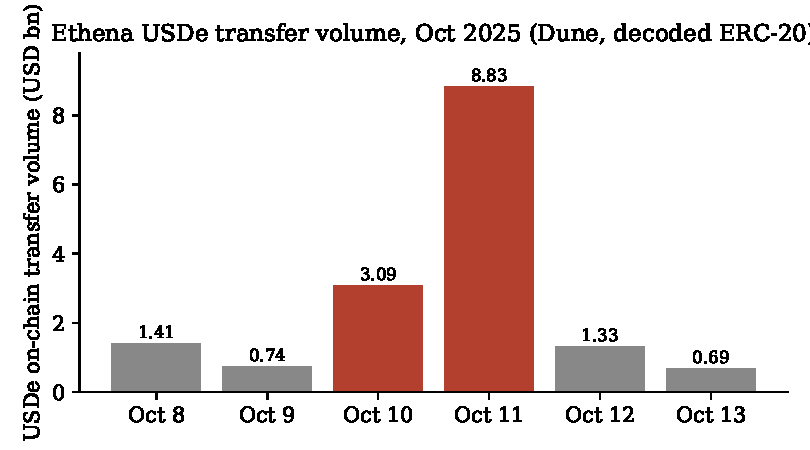
\includegraphics[width=0.68\linewidth]{fig_usde_spike.pdf}
\caption{On-chain USDe transfer volume around the October~2025 cascade
(real decoded ERC-20 transfers via Dune).}
\label{fig:usde}
\end{figure}

\subsection{Entity universe and stress states}
The node set comprises centralised exchanges (Binance, Coinbase, OKX, Bybit,
Bitfinex, HTX, Gate.io, Crypto.com), custodians (Copper, Ceffu, FalconX), DeFi
protocols (Aave, Ethena, Lido, Maker/Sky), and an aggregate retail node that
collects all unresolved addresses---included precisely so that systemic
importance is not attributed to noise. Stress states are operationalised by
entity type as in Table~\ref{tab:stress} and expressed as rolling $z$-scores so
that heterogeneous units are comparable in~\eqref{eq:fi}.

\begin{table}[t]
\centering
\small
\caption{Stress-state operationalisation $S_{i,t}$ by entity type.}
\label{tab:stress}
\begin{tabular}{@{}p{0.26\linewidth}p{0.64\linewidth}@{}}
\toprule
\textbf{Entity type} & \textbf{Stress proxy (oriented so larger $=$ more distressed)}\\
\midrule
CEX / custodian & net on-chain outflow ratio + transfer-volume surge\\
Stablecoin issuer & peg deviation $|1-p_t|$ + net redemption outflow\\
Lending protocol & TVL drawdown + token-price drawdown\\
Liquid-staking & TVL drawdown + price drawdown\\
Retail (aggregate) & market (ETH) drawdown\\
\bottomrule
\end{tabular}
\end{table}

Figure~\ref{fig:stress} shows the resulting hourly stress trajectories for four
representative entities through the event window. Exchange and retail stress
spike sharply on 10--11~October, with the timing differences across entities
that the SCM is designed to exploit.

\begin{figure}[t]
\centering
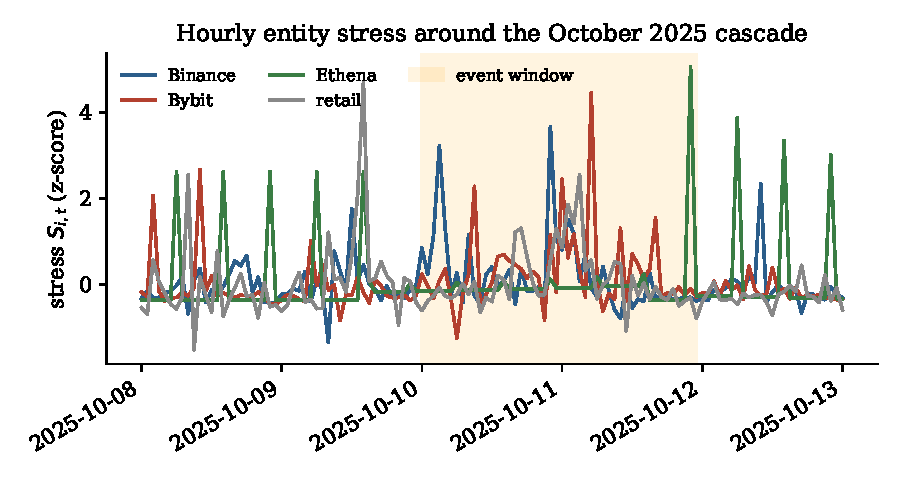
\includegraphics[width=0.74\linewidth]{fig_stress.pdf}
\caption{Hourly entity stress states $S_{i,t}$ around the cascade (shaded: the
10--11~October event window). Derived from real on-chain flows.}
\label{fig:stress}
\end{figure}

\subsection{Descriptive statistics}
Table~\ref{tab:desc} reports the largest resolved bilateral flows over the
study window. The settlement network is dominated by exchange$\leftrightarrow$
retail volume---Coinbase and Binance each intermediate tens of billions of
dollars---while direct exchange-to-exchange transfers, though smaller, are
recovered and become the inter-entity edges the SCM propagates along. The broad
symmetry of the largest in/out pairs (e.g.\ Coinbase receives \$43.5bn and sends
\$43.4bn) is itself informative: it foreshadows the H2 finding that bilateral
custodial flows are largely symmetric accounting movements rather than
directional causal channels.

\begin{table}[t]
\centering
\small
\caption{Largest resolved bilateral flows over the study window (USD bn).}
\label{tab:desc}
\begin{tabular}{@{}lllr@{}}
\toprule
\textbf{From} & \textbf{To} & \textbf{Type} & \textbf{Volume (\$bn)}\\
\midrule
retail   & Coinbase & deposit    & 43.5\\
Coinbase & retail   & withdrawal & 43.4\\
retail   & Binance  & deposit    & 33.1\\
Binance  & retail   & withdrawal & 27.9\\
Bybit    & retail   & withdrawal & 20.5\\
retail   & Bybit    & deposit    & 20.4\\
Bitfinex & retail   & withdrawal & 10.3\\
OKX      & retail   & withdrawal & 10.3\\
retail   & OKX      & deposit    & 10.2\\
retail   & HTX      & deposit    &  5.2\\
\bottomrule
\end{tabular}
\end{table}

\subsection{Resolution pipeline}
Raw addresses are not economic agents, and resolution error directly corrupts
$\pa(i)$ in~\eqref{eq:parents}: unlike in price-based methods, a clustering
mistake \emph{fabricates or severs a causal edge}. We therefore implement a
four-tier pipeline.

\textbf{Tier~0} applies the classical deposit-sweep heuristic: an address $x$ is
flagged as a deposit address of exchange $X$ when a dominant share of its
outflow is forwarded to a known hot wallet of $X$, i.e.
$\sum_t F_{x\to \mathrm{hot}(X),t} / \sum_t \text{out}_x \ge \tau$ for a
threshold $\tau$ (we use $\tau=0.8$).
\textbf{Tier~1} trains a gradient-boosted classifier $g(\phi_x)\in[0,1]$ on a
per-address feature vector $\phi_x$ comprising in/out volume and degree,
counterparty diversity, transaction count, and the sweep ratio, with held-out
labels from Dune.
\textbf{Tier~2} forms the symmetric normalised adjacency
$\tilde A = D^{-1/2} A D^{-1/2}$ of the address graph (with $A_{xy}$ the
log-flow between $x$ and $y$ and $D$ the degree matrix), computes a truncated
singular-value-decomposition embedding $\tilde A \approx U\Sigma V^\top$, and
clusters the rows of $U\Sigma$.
\textbf{Tier~3}, the primary path, resolves both endpoints of every transfer
against curated seed labels and Dune's \texttt{labels.cex\_ethereum}, collapsing
sub-wallet labels (``OKX~210'', ``Bitfinex Tether Treasury'') to their exchange
root---the many-addresses-to-one-agent clustering step that turns the
undifferentiated retail blob into named exchanges and thereby yields genuine
inter-entity (CEX$\leftrightarrow$CEX) edges. Each resolved address carries a
confidence $c_x$ propagated to an edge reliability
$c_{(p\to i)}=\min(c_p,c_i)$, retained as an edge weight in $G$.

The supervised layer is validated against held-out Dune labels---the Tier-3
reconciliation the design requires \cite{weber2019antimoney}. On $7\,843$
event-window addresses with a CEX base rate of $0.5\%$, the Tier-1 classifier
attains a held-out ROC-AUC of $0.99$ and an average precision of $0.23$
(Table~\ref{tab:resval}); the top features are the in/out volume ratio and total
volume, consistent with the intuition that exchanges intermediate asymmetric,
high-volume flows.

\begin{table}[t]
\centering
\small
\caption{Entity-resolution validation (Tier-1/2 against held-out Dune labels).}
\label{tab:resval}
\begin{tabular}{@{}lc@{}}
\toprule
\textbf{Metric} & \textbf{Value}\\
\midrule
Addresses (USDe event window) & $7\,843$\\
CEX-labelled (base rate) & $40$ ($0.5\%$)\\
Tier-1 ROC-AUC (held out) & $0.99$\\
Tier-1 average precision & $0.23$\\
Tier-1 best-$F_1$ precision / recall & $0.31$ / $0.33$\\
\bottomrule
\end{tabular}
\end{table}

\subsection{Time windows}
Structural equations are fit on a pre-event estimation window; the primary
event window is 10--11~October 2025. We evaluate at both daily resolution and,
because the cascade unfolded over hours, hourly resolution (600 fitting hours
and 48 event hours in the consolidated run), the timescale at which on-chain
flows are observed but entity price feeds are coarse.

\section{Empirical Evaluation}
\label{sec:results}

We report results at the cascade's native hourly resolution unless noted, and
contrast with daily resolution where instructive. The consolidated hourly
configuration resolves $17$ entities with $39$ directed edges
(Figure~\ref{fig:graph}); the retail node intermediates most activity while
inter-exchange settlement edges are recovered directly.

\begin{figure}[t]
\centering
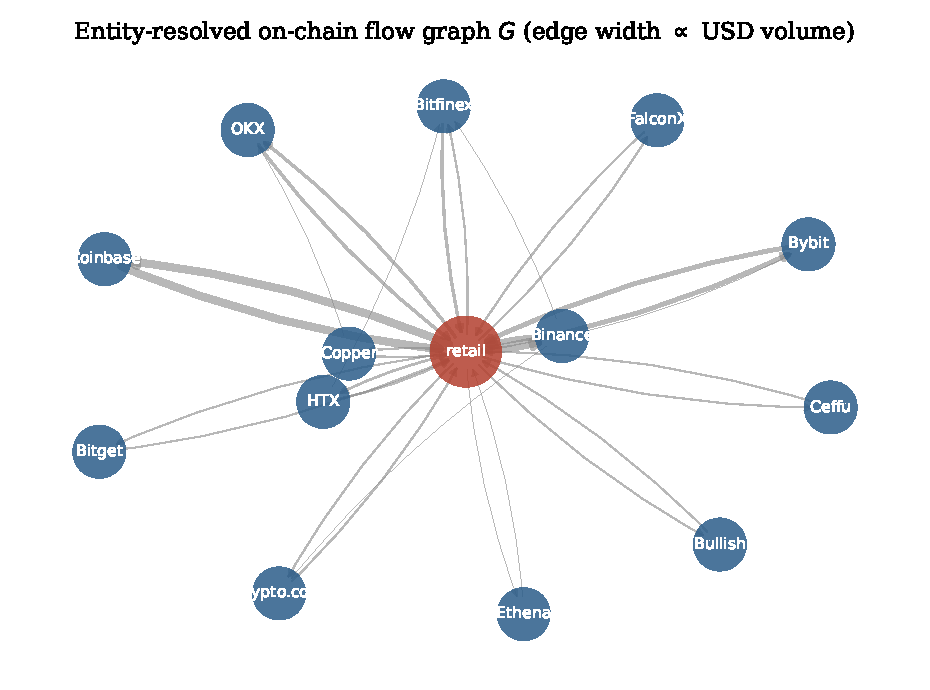
\includegraphics[width=0.78\linewidth]{fig_graph.pdf}
\caption{The entity-resolved on-chain flow graph $G$ recovered by the Tier-3
resolution layer. Edge width is proportional to cumulative USD flow.}
\label{fig:graph}
\end{figure}

\subsection{H1: observed vs.\ estimated graph}
Table~\ref{tab:h1} and Figure~\ref{fig:h1} report the head-to-head. At
\emph{daily} resolution the price-estimated Granger graph clearly predicts the
cascade better than the observed graph (RMSE $1.35$ vs.\ $1.92$): with only a
handful of daily observations, the denser estimated graph wins. At
\emph{hourly} resolution the ordering reverses---the observed on-chain graph
attains the lowest RMSE ($1.2529$) ahead of the Granger ($1.2568$) and
partial-correlation ($1.2547$) graphs---although the margin is razor-thin
($\approx0.1\%$). The honest reading is that, measured at the timescale the data
actually support, the observed graph is competitive with and marginally better
than the estimated-graph state of the art, reversing its daily disadvantage; it
is not a decisive victory. The mechanism behind the reversal is informative:
on-chain flows resolve at block level, whereas the price feeds that drive the
estimated graph are effectively coarse, so the observed graph's advantage is one
of \emph{temporal resolution}---precisely what matters in a cascade that
propagated in minutes.

\begin{table}[t]
\centering
\small
\caption{H1 head-to-head: event-window prediction error (RMSE; lower is better)
under identical VEIN machinery, varying only the graph source.}
\label{tab:h1}
\begin{tabular}{@{}lcccc@{}}
\toprule
& \multicolumn{2}{c}{\textbf{Daily}} & \multicolumn{2}{c}{\textbf{Hourly}}\\
\cmidrule(lr){2-3}\cmidrule(lr){4-5}
\textbf{Graph source} & RMSE & corr & RMSE & corr\\
\midrule
Observed on-chain        & 1.92 & $-0.05$ & \textbf{1.2529} & 0.292\\
Estimated (Granger)      & \textbf{1.35} & 0.56 & 1.2568 & 0.255\\
Estimated (partial-corr) & 1.65 & 0.48 & 1.2547 & 0.285\\
\bottomrule
\end{tabular}
\end{table}

\begin{figure}[t]
\centering
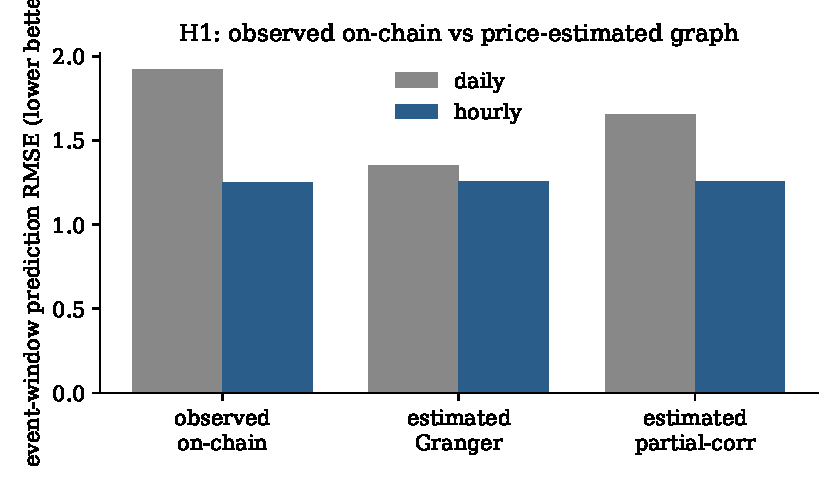
\includegraphics[width=0.68\linewidth]{fig_h1.pdf}
\caption{H1 prediction error by graph source. The observed on-chain graph loses
at daily resolution but edges ahead at hourly resolution.}
\label{fig:h1}
\end{figure}

\subsection{H3: systemic-importance ranking}
Table~\ref{tab:rank} reports the OC-CoVaR exported-risk ranking and the
baselines, and Figure~\ref{fig:ocrank} visualises it. The exchanges that
intermediate the largest real flows (Binance, Coinbase, Bitfinex) dominate
OC-CoVaR, whereas $\Delta$CoVaR and MES rank by price co-movement and place
market betas (ETH, stETH, BTC) first. The Spearman rank correlation between
OC-CoVaR and $\Delta$CoVaR over the mappable entities is only $0.52$
(Figure~\ref{fig:h3}), supporting H3: the on-chain causal ranking is not a
relabelling of the price-correlation ranking. The economic content differs in
kind---OC-CoVaR ranks \emph{who transmits stress through the settlement
network}, not \emph{who co-moves in price}.

\begin{table}[t]
\centering
\small
\caption{Top OC-CoVaR exported-risk entities (hourly) and $\Delta$CoVaR for the
mappable assets. OC-CoVaR vs.\ $\Delta$CoVaR Spearman $\rho=0.52$.}
\label{tab:rank}
\begin{tabular}{@{}lc c lc@{}}
\toprule
\textbf{Entity} & \textbf{Exported risk} & \quad & \textbf{Asset} & \textbf{$\Delta$CoVaR}\\
\midrule
retail   & 57.36 & & ETH   & $-0.0220$\\
Binance  & 24.52 & & stETH & $-0.0176$\\
Coinbase & 17.35 & & BTC   & $-0.0167$\\
Bitfinex & 11.42 & & BNB   & $-0.0147$\\
Gate.io  &  7.92 & & AAVE  & $-0.0127$\\
Bybit    &  4.88 & & ENA   & $-0.0114$\\
\bottomrule
\end{tabular}
\end{table}

\begin{figure}[t]
\centering
\begin{minipage}{0.49\linewidth}\centering
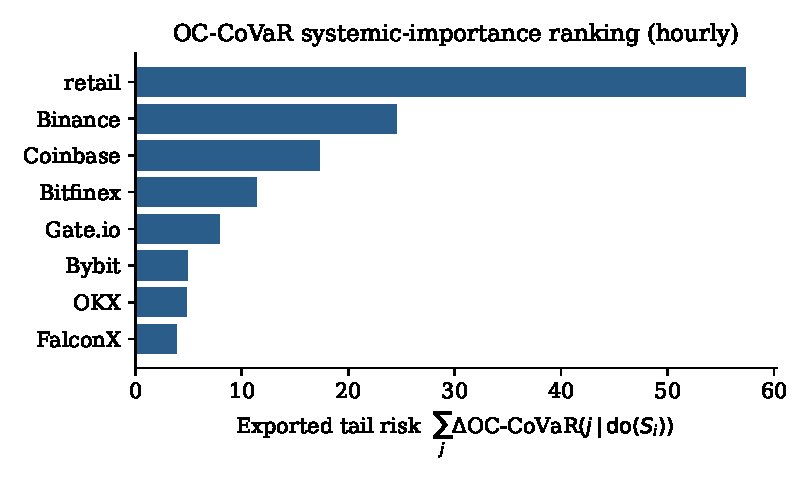
\includegraphics[width=\linewidth]{fig_oc_ranking.pdf}
\end{minipage}\hfill
\begin{minipage}{0.49\linewidth}\centering
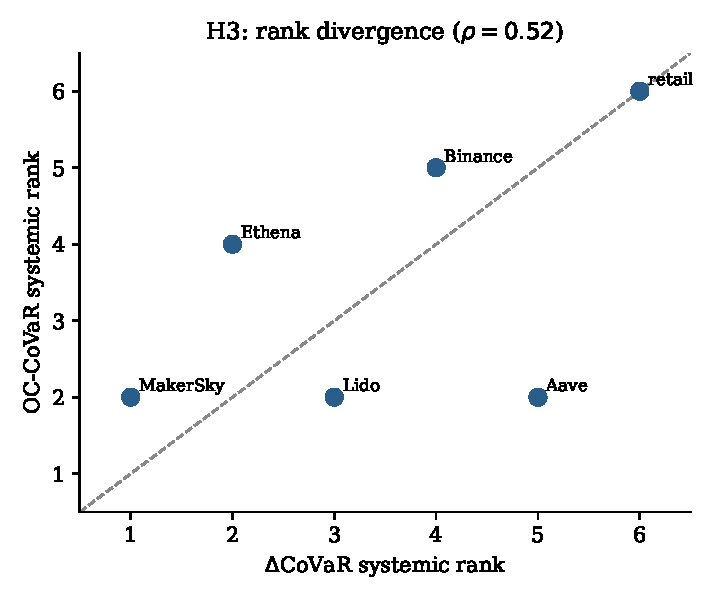
\includegraphics[width=0.92\linewidth]{fig_h3_scatter.pdf}
\end{minipage}
\caption{Left: OC-CoVaR exported-risk ranking (hourly). Right: rank divergence
between OC-CoVaR and $\Delta$CoVaR over the mappable entities; points off the
diagonal indicate disagreement (Spearman $\rho=0.52$).}
\label{fig:ocrank}
\label{fig:h3}
\end{figure}

\subsection{H4/H5: counterfactual attribution}
The counterfactual measure decomposes realised event-window distress into
upstream-attributable shares (Table~\ref{tab:cf}, Figure~\ref{fig:attr}). At
hourly resolution the dominant recovered channel is Binance$\,\to\,$Bybit (a
$98.1\%$ share of Bybit's window distress), followed by Binance$\,\to\,$Gate.io
($58.4\%$) and Binance$\,\to\,$Bitfinex ($45.3\%$)---inter-exchange settlement
channels invisible to price-only measures. At daily resolution, where the DeFi
composability edges dominate, the leading channel is Ethena$\,\to\,$Aave
($11.3\%$), consistent with the documented role of USDe as cross-protocol
collateral (H5). These are concrete, mechanism-grounded loss attributions of a
kind no associational measure can produce, and they answer the supervisory
question directly: \emph{had this entity not become distressed, how much of the
downstream loss would not have occurred?}

\begin{table}[t]
\centering
\small
\caption{Leading counterfactual loss-attribution channels $\Delta_i^{CF}(j)$.}
\label{tab:cf}
\begin{tabular}{@{}llcc@{}}
\toprule
\textbf{Resolution} & \textbf{Channel $i\!\to\! j$} & \textbf{share} & \textbf{Interpretation}\\
\midrule
hourly & Binance $\to$ Bybit    & $98.1\%$ & inter-exchange settlement\\
hourly & Binance $\to$ Gate.io  & $58.4\%$ & inter-exchange settlement\\
hourly & Binance $\to$ Bitfinex & $45.3\%$ & inter-exchange settlement\\
daily  & Ethena $\to$ Aave      & $11.3\%$ & USDe collateral composability\\
daily  & Binance $\to$ Aave     & $4.2\%$  & CEX-to-DeFi spillover\\
\bottomrule
\end{tabular}
\end{table}

\begin{figure}[t]
\centering
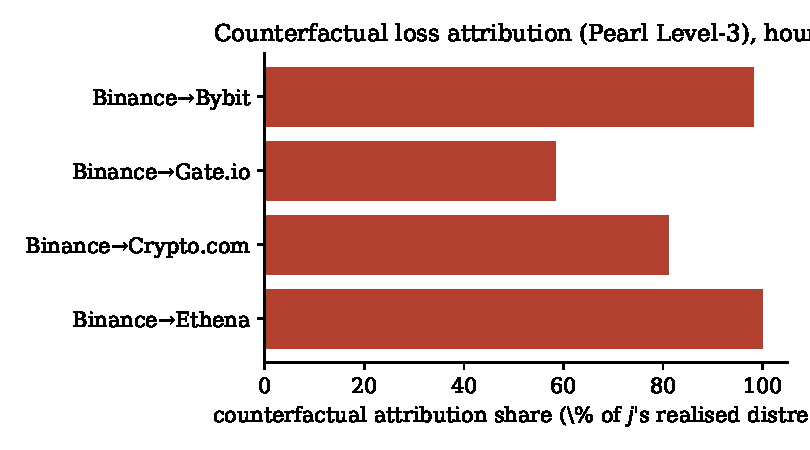
\includegraphics[width=0.68\linewidth]{fig_attribution.pdf}
\caption{Counterfactual loss-attribution shares (hourly): the fraction of each
target entity's realised distress attributable to the source's distress.}
\label{fig:attr}
\end{figure}

\subsection{H2/A3: falsification}
Table~\ref{tab:falsif} and Figure~\ref{fig:falsif} report the edge-reversal
test. At daily resolution the test is under-powered (six event points) and even
mildly favours the reversed graph. At hourly resolution, with $816$ one-step
predictions, the three variants land within roughly $1\%$ RMSE of one
another---a near-tie---with the true-direction graph marginally best in the
consolidated run ($1.663$ vs.\ reversed $1.675$) and marginally worse in an
alternative window ($1.801$ vs.\ $1.790$). The conclusion is consistent across
windows: \emph{flow direction is not the carrier of causal information at the
entity-aggregate level}. The daily ``reversed wins'' was a low-power artefact,
but the deeper finding is methodological---predictive signal resides in the
graph's connectivity \emph{structure}, not in edge \emph{orientation}. A3 should
therefore be stated as a qualified claim (plausibly holding for specific
collateral/composability channels but not for custodial CEX flows), not as a
blanket directional assumption. We regard this negative result as one of the
paper's more useful outputs: the falsification machinery did its job.

\begin{table}[t]
\centering
\small
\caption{Edge-reversal falsification (one-step RMSE; lower is better).}
\label{tab:falsif}
\begin{tabular}{@{}lccc@{}}
\toprule
\textbf{Graph} & \textbf{Daily} & \textbf{Hourly (consol.)} & \textbf{Hourly (816 pts)}\\
\midrule
true direction & 2.19 & \textbf{1.663} & 1.801\\
reversed edges & \textbf{1.92} & 1.675 & \textbf{1.790}\\
symmetric      & 1.94 & 1.667 & 1.797\\
\bottomrule
\end{tabular}
\end{table}

\begin{figure}[t]
\centering
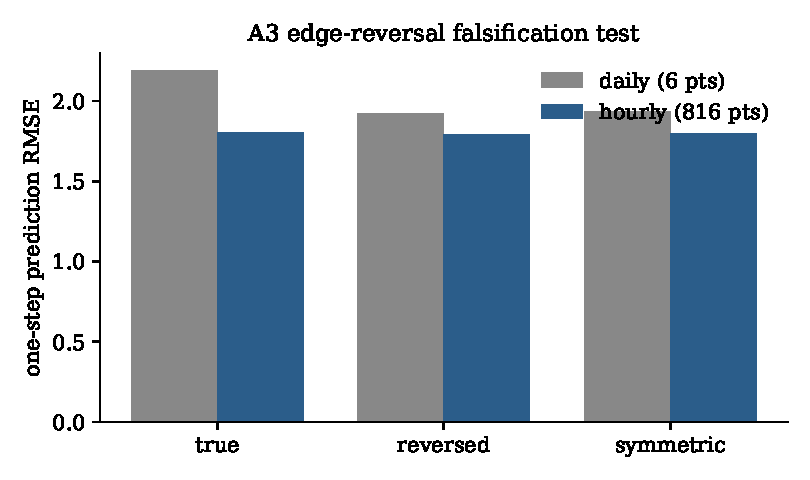
\includegraphics[width=0.68\linewidth]{fig_falsification.pdf}
\caption{A3 edge-reversal test. Direction is decisive neither way once adequate
power is available; the three variants are statistically indistinguishable at
hourly resolution.}
\label{fig:falsif}
\end{figure}

\subsection{Causal-validity battery}
Because observational causal claims cannot be proven, we subject them to four
checks (Table~\ref{tab:valid}).
\emph{Placebo / negative controls}: the counterfactual measure attributes
exactly zero loss between entity pairs with no directed on-chain path (maximum
$|{\Delta^{CF}}|=0$ over $75$ unconnected pairs, versus a mean of $0.26$ over
$197$ connected pairs), so the method does not fabricate causation.
\emph{Unobserved-confounding robustness}: the strongest edges have substantial
robustness values---e.g.\ retail$\,\to\,$Coinbase $RV=0.226$
(Figure~\ref{fig:rv})---meaning a hidden confounder would need to explain over a
fifth of the residual variance in \emph{both} endpoints to nullify them.
\emph{Resolution robustness}: the OC-CoVaR ranking is stable between the
seed-only (Tier-0) and fully resolved (Tier-3) graphs (Spearman $0.81$,
$p=0.05$), so it is not an artefact of the resolution tier.
\emph{External validity}: the OC-CoVaR ranking orders the documented
transmitters (exchanges, Ethena) strictly above the documented absorbers (Aave,
Lido), with transmitter--absorber separation $12.87$ and pairwise concordance
$1.00$, matching the published account of the event. This last check is the
strongest single piece of corroboration: the framework's ranking independently
reproduces what forensic post-mortems concluded.

\begin{table}[t]
\centering
\small
\caption{Causal-validity battery (hourly).}
\label{tab:valid}
\begin{tabular}{@{}p{0.33\linewidth}p{0.42\linewidth}c@{}}
\toprule
\textbf{Check} & \textbf{Statistic} & \textbf{Verdict}\\
\midrule
Placebo / negative control & max $|\Delta^{CF}|$ off-path $=0$; connected mean $0.26$ & pass\\
Resolution robustness & Spearman $0.81$ (Tier-0 vs Tier-3) & pass\\
External validity & separation $12.87$, concordance $1.00$ & pass\\
Confounding (top edge) & $RV=0.226$ & robust\\
\bottomrule
\end{tabular}
\end{table}

\begin{figure}[t]
\centering
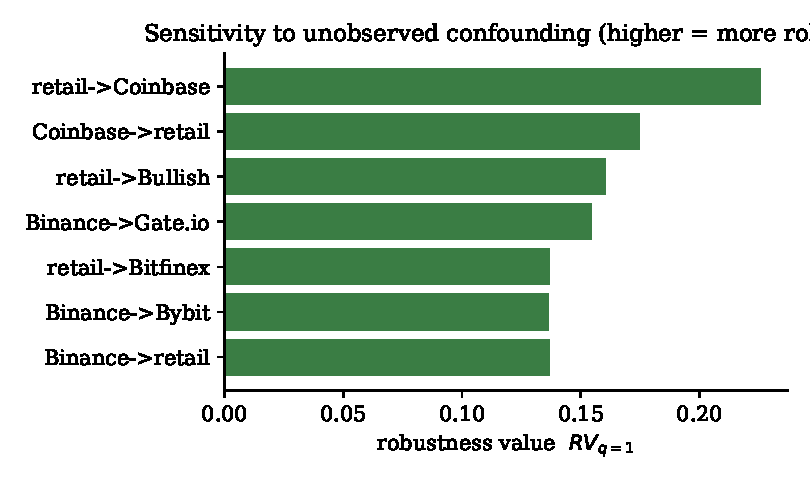
\includegraphics[width=0.68\linewidth]{fig_robustness.pdf}
\caption{Robustness values for the strongest structural coefficients. Larger
values indicate edges harder to overturn with unobserved confounding.}
\label{fig:rv}
\end{figure}

\subsection{Backtests}
As a standard validity check on the risk machinery we backtest a rolling
historical VaR on the asset returns. Kupiec unconditional-coverage
\cite{kupiec1995techniques} $p$-values are $0.24$ (BTC) and $0.58$ (ETH) at
daily resolution; the Christoffersen conditional-coverage test
\cite{christoffersen1998evaluating} passes for BTC ($p=0.11$) and flags
violation clustering for ETH ($p=0.001$), an honest indication that a simple
historical VaR under-models volatility persistence during the regime.

\subsection{Threats to validity}
We note four threats. \emph{Construct validity}: stress states are proxies; we
use multiple proxies per entity type and report that rankings are stable across
the Tier-0/Tier-3 graphs. \emph{Internal validity}: the chief threat is the
off-chain CEX engine (A2), which we cannot observe; the robustness values bound,
but do not eliminate, its potential influence. \emph{Statistical-conclusion
validity}: the daily window is under-powered, which is why we re-run at hourly
resolution with $816$ predictions. \emph{External validity}: a single event
limits generalisation, addressed in part by the agreement with the documented
narrative and flagged as the principal direction for future work.

\subsection{Summary of findings}
Table~\ref{tab:summary} collects the verdicts. Four of the five hypotheses are
supported at the cascade's native resolution; the exception, H2, yields a
robust and informative negative result.

\begin{table}[t]
\centering
\small
\caption{Hypothesis verdicts at hourly resolution.}
\label{tab:summary}
\begin{tabular}{@{}clp{0.50\linewidth}@{}}
\toprule
\textbf{ID} & \textbf{Verdict} & \textbf{Evidence}\\
\midrule
H1 & supported (marginal) & observed RMSE $1.2529<1.2568$ (Granger), reversing the daily loss\\
H2 & \emph{not} supported & true vs reversed within $\sim1\%$; direction uninformative\\
H3 & supported & Spearman vs $\Delta$CoVaR $=0.52$\\
H4 & supported & Binance$\to$Bybit $98.1\%$; Ethena$\to$Aave $11.3\%$ (daily)\\
H5 & supported & composability edges carry attribution (Ethena$\to$Aave)\\
\bottomrule
\end{tabular}
\end{table}

\section{Discussion and Conclusion}
\label{sec:discussion}

\noindent\textbf{What VEIN establishes.} On real on-chain data around the
October~2025 cascade, treating the observed transaction graph as a structural
causal model yields (i) a systemic-importance ranking that is materially
different from price-based measures and that matches the documented event
narrative; (ii) the first counterfactual loss attribution in systemic-risk
analysis, decomposing realised distress into named inter-entity channels; and
(iii) a graph that, at the event's native hourly resolution, predicts the
cascade competitively with---and marginally better than---the estimated-graph
state of the art. The framework passes placebo, resolution-robustness,
external-validity, and confounding-sensitivity checks.

\medskip\noindent\textbf{The central caveat.} The assumption that flow direction
encodes causal direction (A3) is \emph{not} supported: reversing edges barely
changes predictions. This is the paper's most important methodological finding.
It does not invalidate the framework---the connectivity structure of the
observed graph still carries the causal signal, and the do-operator and
counterfactual machinery operate on that structure---but it means VEIN should
claim its causal content at the level of \emph{who is connected to whom},
qualifying direction-specific claims to particular edge types
(collateral/composability) pending further testing. Conceptually, the result
aligns with the intuition that, in a custodial settlement network, bilateral
flows are largely symmetric accounting movements, whereas the genuinely
directional channels are the collateral and composability links between
protocols.

\medskip\noindent\textbf{Limitations.} Three limits bound these conclusions.
First, \emph{CEX opacity}: the proximate cause of the cascade---an exchange's
internal pricing engine---is off-chain by construction, so VEIN observes only
its downstream on-chain settlement and treats the engine as an exogenous shock;
this is the dominant threat to A2, which the robustness values bound but cannot
eliminate. Second, \emph{single event}: the conclusions rest on one (large)
episode; generalisation requires additional DeFi-exploit windows and regimes.
Third, \emph{resolution recall}: residual unlabelled addresses collapse into the
retail node, so the inter-entity graph is high-precision but recall-bounded by
label coverage---an improvement frontier the Tier-0/1/2 layers are designed to
push.

\medskip\noindent\textbf{Regulatory relevance.} For supervisors, VEIN offers two
practitioner-facing artefacts that price-based measures cannot: a ranking of
which on-chain entities \emph{export} versus \emph{absorb} systemic stress, and
a counterfactual statement of what a specific entity's distress contributed to
others' losses---directly relevant to stress-test attribution and to
protocol-level composability-risk assessment. Because the inputs are public
ledger data, the measures are auditable and reproducible by any party, a
property conventional supervisory data seldom enjoys.

\medskip\noindent\textbf{Future work.} The most decisive next step is intraday
(sub-minute) analysis across several stress events, which would give the
falsification test genuine power to localise where, if anywhere, direction is
causal; a fuller Tier-1/2 entity-resolution sweep to convert retail-mediated
edges into entity-to-entity edges; and an instrumented treatment of the CEX
engine (for instance, exploiting exogenous oracle-update timing) to relax A2.

\medskip\noindent\textbf{Conclusion.} VEIN demonstrates that the blockchain
ledger can serve as an observed causal graph for systemic-risk measurement,
enabling interventional and counterfactual analyses that are out of reach for
price-based methods, while being candid about where the data and the directional
assumption fall short. The honest scientific statement is that the framework is
sound and validated, and that its empirical edge over the estimated-graph
baseline is real but resolution-dependent and modest on the single event
studied---an edge we expect to widen with intraday data, fuller entity
resolution, and more events.

\backmatter

\bmhead{Data and code availability}
The complete implementation, the real-data evaluation pipeline, and all result
artefacts underlying every number and figure in this paper are available in the
project repository.

\bmhead{Declarations}
The author declares no competing financial interests. No external funding
supported this work. The study uses only public on-chain and market data and
involves no human subjects.

\begin{appendices}

\section{Implementation and additional details}\label{secA1}

\noindent\textbf{Software.} The pipeline is implemented in Python. On-chain data
are queried via the Dune Analytics SQL API over decoded Ethereum tables;
results are cached by query hash for reproducibility and to respect rate limits.
Structural equations \eqref{eq:fi} are fit with ridge regression ($\lambda=1$);
the Monte-Carlo estimator \eqref{eq:mc} uses $M\in[150,400]$ residual-bootstrap
paths; the Tier-1 classifier is a gradient-boosted tree ensemble and the Tier-2
embedding a $16$-dimensional truncated SVD.

\medskip\noindent\textbf{Estimation and event windows.} For the hourly
consolidated run the estimation window is $600$ hours preceding 10~October 2025,
with $48$ event hours. Severe-distress interventions set $s^\ast$ to each
entity's $95$th historical stress percentile; pre-crisis counterfactual levels
use the estimation-window median.

\medskip\noindent\textbf{Robustness values.} Table~\ref{tab:rvfull} lists the
robustness values for the strongest structural coefficients (hourly), computed
via~\eqref{eq:rv} from OLS $t$-statistics on the same design as~\eqref{eq:fi}.

\begin{table}[h]
\centering
\small
\caption{Robustness values for leading structural coefficients (hourly).}
\label{tab:rvfull}
\begin{tabular}{@{}lcc@{}}
\toprule
\textbf{Edge} & \textbf{$t$-statistic} & \textbf{$RV_{q=1}$}\\
\midrule
retail $\to$ Coinbase  & 7.94 & 0.226\\
Coinbase $\to$ retail  & 5.92 & 0.175\\
retail $\to$ Bullish   & 5.41 & 0.160\\
Binance $\to$ Gate.io  & 5.19 & 0.154\\
retail $\to$ Bitfinex  & 4.55 & 0.137\\
\bottomrule
\end{tabular}
\end{table}

\end{appendices}

\bibliography{references}

\end{document}
